\documentclass[aps,pre,12pt,preprint,%
	onecolumn,showpacs,showkeys,nofootinbib]{revtex4-2}
%Chinese
	\usepackage[UTF8,fontset=fandol]{ctex}
%	\usepackage[datesep=/]{datetime2} % Use default
	\DeclareTextFontCommand{\textbf}{\sffamily}
%Presenting
	\usepackage[table]{xcolor}
	\usepackage{graphicx}
	\usepackage[font=small,format=plain,%
		labelfont=bf,textfont=it,%
		singlelinecheck=false]{caption}
	\usepackage[above]{placeins}
%	\usepackage{float} % Cause trouble for table footnotes
	\usepackage{wrapfig}
	\usepackage{tabularx,array,booktabs,multirow,bigstrut}
	\newcolumntype{C}[1]{>{\hsize=#1\hsize%
		\centering\arraybackslash}X}
	\newcommand{\minitab}[2][l]{%
		\begin{tabular}{#1}#2\end{tabular}}
	\usepackage{setspace,dcolumn}
	\usepackage{subfig}
	\usepackage{psfrag,epsfig}
%MathSetting
	\let\latexointop\ointop
	\usepackage{amsmath,bm,amssymb,esint,extarrows}
	\usepackage{upgreek,textcomp,mathrsfs}
	\usepackage[only,sslash]{stmaryrd}
	\usepackage{nicefrac,eqnarray}
%	\usepackage{amsthm} % Enable when necessary
%	\usepackage[mathscr]{eucal} % Enable when necessary
	\usepackage{mathtools,physics,siunitx}
	\usepackage{stackengine,varwidth}
	\usepackage{tikz}
	\usepackage{resizegather,empheq}
	\usetagform{default}
	\usepackage{calligra,fourier-orns}
	% Keep \oint unchanged by esint
	\let\ointop\undefined
	\let\ointop\latexointop
	% Define a scriptr 
	\DeclareMathAlphabet{\mathcalligra}{T1}{calligra}{m}{n}
	\DeclareFontShape{T1}{calligra}{m}{n}{<->s*[2.2]callig15}{}
	\newcommand{\scriptr}{\mathcalligra{r}\,}
	\newcommand{\rvector}{\pmb{\mathcalligra{r}}\,}
	% Useful shorthand
	\DeclarePairedDelimiter\ave{\langle}{\rangle}
	\newcommand\inlineeqno{\stepcounter{equation}\ (\theequation)}
	\newcommand{\sinc}{\operatorname{sinc}}
	\newcommand{\mbb}[1]{\mathbb{#1}}
	\newcommand{\mrm}[1]{\mathrm{#1}}
	\newcommand{\mcal}[1]{\mathcal{#1}}
	% Scaling and positioning
	\newcommand\scalemath[2]{\scalebox{#1}{\mbox{\ensuremath{\displaystyle #2}}}}
	\newcommand\raisemath[2]{\raisebox{#1\depth}{${#2}$}}
	\empheqset{box=\nicebox}
	% Presenting
	\newcommand*\nicebox[1]{\fbox{\hspace{1em}\addstackgap[5pt]{#1}\hspace{1em}}}

	\allowdisplaybreaks[2]
%ParagraphSetting
	\setlength{\parskip}{.3\baselineskip}
	\usepackage[defaultlines=2,all]{nowidow}
	\postdisplaypenalty=50
%PageSetting
	\usepackage{titlesec}
	\titleformat*{\section}{\large\bfseries}
	\usepackage[colorlinks=true,linkcolor=blue]{hyperref}
	\newcommand{\texstringonly}[1]{%
		\texorpdfstring{#1}{}}
	\usepackage[vmargin={3.5cm,4cm},hmargin=3cm,%
		footnotesep=\baselineskip]{geometry}
%	\usepackage[bottom]{footmisc} % Cause trouble for table footnotes
	\usepackage{changepage}
	% Autoref names
	\renewcommand{\tableautorefname}{\tablename}
	\renewcommand{\figureautorefname}{\figurename}
	% List settings
	\usepackage{enumitem}
	\setlist{itemsep=0pt,topsep=0pt,labelindent=\parindent,leftmargin=0pt,itemindent=*}
	% Some redefined lengths
	\setlength{\headsep}{1.6\baselineskip}
%	\setlength{\footnotesep}{3\parskip} % Use when necessary
	% Header
	\usepackage{fancyhdr,lastpage}
	\pagestyle{fancy}
%	\fancyhf{} % Clear default settings; disabled for now
	\cfoot{--\ \thepage\,/\,\pageref{LastPage} \ --}
	\setlength{\footskip}{2\baselineskip}
	\renewcommand{\headrulewidth}{0.1pt}
	\renewcommand{\headrule}{
		\ifnum\value{page}=1\relax\else
			\vbox to 2pt{
			\hbox to \headwidth{\dotfill}\vss}
		\fi}
	\fancypagestyle{titlepagestyle}{%
		\fancyhead{}
		\chead{
			\vspace{2.5\baselineskip}
			
\includegraphics[width=.75\linewidth]{../PKUPhy}}
	}
	% Separator
	\newcommand{\newparagraph}{\pagebreak[3]\noindent%
		\hfil
		~\raisebox{-4pt}[10pt][10pt]{\decofourright~~~~~~~~\decofourleft}~ %
		\par
	}
%	% Background % Use when necessary
%	\usepackage{background} %Waterstamp package
%	\SetBgContents{...的实验报告} %Waterstamp to prevent copying
%	\SetBgScale{5} %Waterstamp setting
	% Essay format
	\renewcommand\appendixname{附录}
	\renewcommand\abstractname{}
	\renewcommand\tablename{表}
	\renewcommand\figurename{图}
	\renewcommand\refname{参考文献}
	\renewcommand\contentsname{目录}
	\makeatletter
	\def\@pacs@name{\songti\zihao{-4}{\bf PACS码:}}
	\def\@keys@name{\songti\zihao{-4}{\bf 关键词:}}
	\def\Dated@name{日期:}
	\def\Received@name{\zihao{-5}{接收} }
	\def\Revised@name{\zihao{-5}{修订} }
	\def\Accepted@name{\zihao{-5}{采纳} }
	\def\Published@name{\zihao{-5}{发表} }
	\makeatother
	\linespread{1.5}
	\renewcommand{\labelenumi}{\alph{enumi}.}
	\leftmargini=20mm
	\newcommand{\supercite}[1]{\textsuperscript{\,%
		[\citenum{#1}]}}
	\let\fancycite\cite
	\renewcommand{\cite}[1]{\textup{\fancycite{#1}}}

%Miscellaneous
%	\newcommand{\tabindent}{\hspace{2em}}
%FourierTransform
	\newcommand{\fourierf}{\mathscr F}
\begin{document}
%Basic Data
	\title{%
	\texstringonly{\hfil\\[2\baselineskip]}
	\sf\LARGE%
		泵浦探测光路搭建%
	\texstringonly{\vspace{3ex}}}
	\author{\fangsong\large%
		吴熙楠%
	\vspace{2mm}}
	\affiliation{\it%
		北京大学物理学院~~学号:\normalfont 1900011413\,}
	\date{\today}
	\keywords{泵浦探测技术,超快激光,自相关技术}
	\email{xinanwu@pku.edu.cn;}
	
\begin{abstract}
\vspace{10mm}
\begin{spacing}{1.5}\normalsize
\setlength{\parskip}{.3\baselineskip}
%	200—300字,
%	说明用什么方法做了什么事,
%	由此得到什么结果和结论,
%	有何意义. 
%	不用缩略词,不用第一人称.
%	
在本实验中学习了泵浦探测的原理, 并搭建了用于泵浦探测实验的光路, 实现了可调节的延时线, 为以后搭建类似的光路提供了训练和思路.
\end{spacing}
\end{abstract}
\clearpage
\maketitle
\thispagestyle{titlepagestyle}
%
%	\item 课程实验报告应假定读者既不是已知全部实验细节的指导教师,也不是缺少专业知识的公众,而是同领域的实验研究者,或审稿人. 不能要求读者要在读过课程讲义后才能读懂课程实验报告.
%	\item 公式、图和表要分别用阿拉伯数字编列序号. 公式和图表要达到可发表的质量.
%	\item 凡不是自己独立思考得到的内容都应该引参考文献. 不能大段引用同一参考文献. 对复杂问题,应该优先考虑引用参考文献得到结果. 对简单一些的问题才鼓励独立思考.
%	\item 较长的推导和说明可以作为附件提交,不占用报告篇幅.
%	\item 思考题不是报告的组成部分. 应另起一页附在报告的最后.

\newpage
\section{引言}
%	研究论文引言一般包含以下内容:
%	(1)所研究领域背景和现状;
%	(2)有待研究的问题;
%	(3)本研究的目的、主要内容和结果;
%	(4)结果的意义.\par
%	在写实验报告的引言时,同学可以假想自己是第一个做类似研究的人.\par
%	引言一定要切合报告正文,不能漫无目的地介绍背景. 要快速地将读者引导到报告主题上,并作较深入的讨论.\par
%	引言篇幅可以在较大范围内变化,但最长不应超过报告文字篇幅的1/3.\par
%	引言撰写可以参考实验讲义,可以复述,但不能复制讲义上的任何一句话.\par
%%%%%%%%%%%%%%%%%%%%%%%%%%%%%%
超快激光领域, 脉冲宽度不断变窄, 激光脉冲已达到几个fs量级. 但即使是最快的光电探测器和带宽示波器的响应时间也有几十个 ps, 因而不能用于测量 fs 脉冲激光的脉宽. 因此人们只能利用超短激光脉冲自身来进行测量, 称为自相关测量. 此外, 对于材料的飞秒超快非线性时间响应的动力学过程的测量也只能利用自相关原理设计的泵浦探测技术来测量.

泵浦探测技术的原理: 用一束短脉冲激光来激发材料, 材料中的超快时间响应的动力学特性可以由一束弱的探测光来测量. 通过改变探测激光对于泵浦激光的时间延迟, 记录探测激光通过样品后的变化, 实验者可以实现对于材料超快动力学过程的探测. 本实验便是对一种泵浦探测光路的搭建.
\section{实验}
%	在此部分需要将实验条件交待清楚到别人能重复你的实验结果的程度. 此外,还需表明你已尽了最大努力来提高实验精度和结果的可靠性. 简单的不确定度估计可以在此节给出,复杂一些的可以放到分析讨论部分.\par
%	实验条件不仅是指直接影响实验结果的实验参量,而且还包括影响实验质量和可靠性的因素,如室温、空气湿度、基真空、原材料纯度等.\par
%	作为教学实验报告,此节写详细一点没有坏处.\par
%	成段有叙述,必要才分节。
%%%%%%%%%%%%%%%%%%%%%%%%%%%%%%
实际实验中人们常常用非共线的泵浦探测技术, 以避免强的泵浦激光对探测系统造成伤害. 典型的非共线泵浦探测技术如图 1 所示. 本次实验中只有一台激光器, 便将其分束, 一束用于泵浦, 另一束较弱的用于探测.
	\begin{figure}[!h]
	\centering
	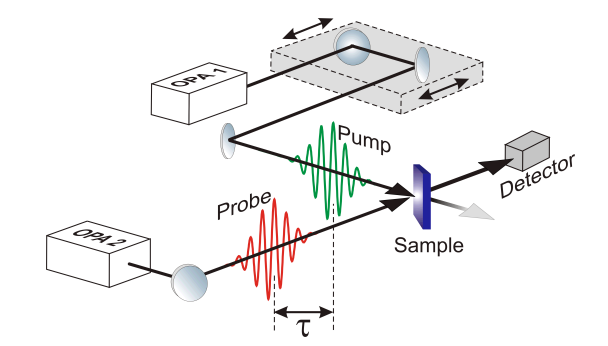
\includegraphics[width=.7\linewidth]{img/1.png}
	\caption[典型的非共线的泵浦探测光路]{典型的非共线的泵浦探测光路}\vspace{1ex}
	\end{figure}
\section{结果与分析}
%	实验结果应尽量以图表的形式给出. 每一个图表都应该是完整的,即阅读图表时可以不必依赖正文.\par
%	依自己意愿,实验结果和对结果的分析讨论既可分为两节也可合在一节.\par
%	\begin{table}[h]
%	\caption{元件恒流大小,为什么要左对齐呢?奇怪。}
%	\small
%	\begin{tabularx}{.6\linewidth}{C{.3} C{1}}
%	\toprule
%	\midrule
%		元件\footnote{%
%			注释一个看看%
%		} & 恒流大小\footnote{%
%			再开一个!哈哈
%		} \\
%	\midrule
%		Pt  &
%			$\SI{1.00005}{\mA}
%				= \SI{100.005}{\mV} / \SI{100}{\ohm} $ \\
%	\midrule
%	\bottomrule
%	\end{tabularx}
%	\label{tab:ExTab}
%	\end{table}
%	
%	每个图一般包含:图名、轴名、轴、刻度、标尺、数据点、曲线、图例、标注和图注等部分. 应尽量让读者不看正文就能基本理解图的含意.\par
%	逐点测量得到的函数关系要同时用表格和图给出. 需要作比较的多条曲线要画在同一图上.\par
%	为避免读者在图表和正文间反复跳跃阅读,在正文中也要对图表作必要的说明.\par
%	
%	对于预料之外的实验结果,必须首先小心证明其可靠性.读者只有在相信你的实验结果时才愿意花时间看你的分析.\par
%	必须用文字归纳整理出正式的实验结果或结论.可信的实验结果是课程报告最重要的内容.作为一个实验物理工作者,分析解释出错并不丢脸,实验结果不被采信则是致命的.\par
%	教学实验的结论往往是预先知道的. 所以,教师更关心的是你的说理过程. 一般说来,单由课内实验的结果不足以能得到明确的结论. 此时,你可以引用他人的研究结果来帮助帮助自己的论证,但必须注明出处. \par
%	确实不能得到明确结论时,可以给出几种可能结论并指出可以再做哪些实验来帮助作进一步的判断.\par
%	总之,分析讨论部分要做到: 论据要valid,论证要reasonable,结论要convincing.\par
%%%%%%%%%%%%%%%%%%%%%%%%%%%%%%
	\begin{figure}[!h]
	\centering
	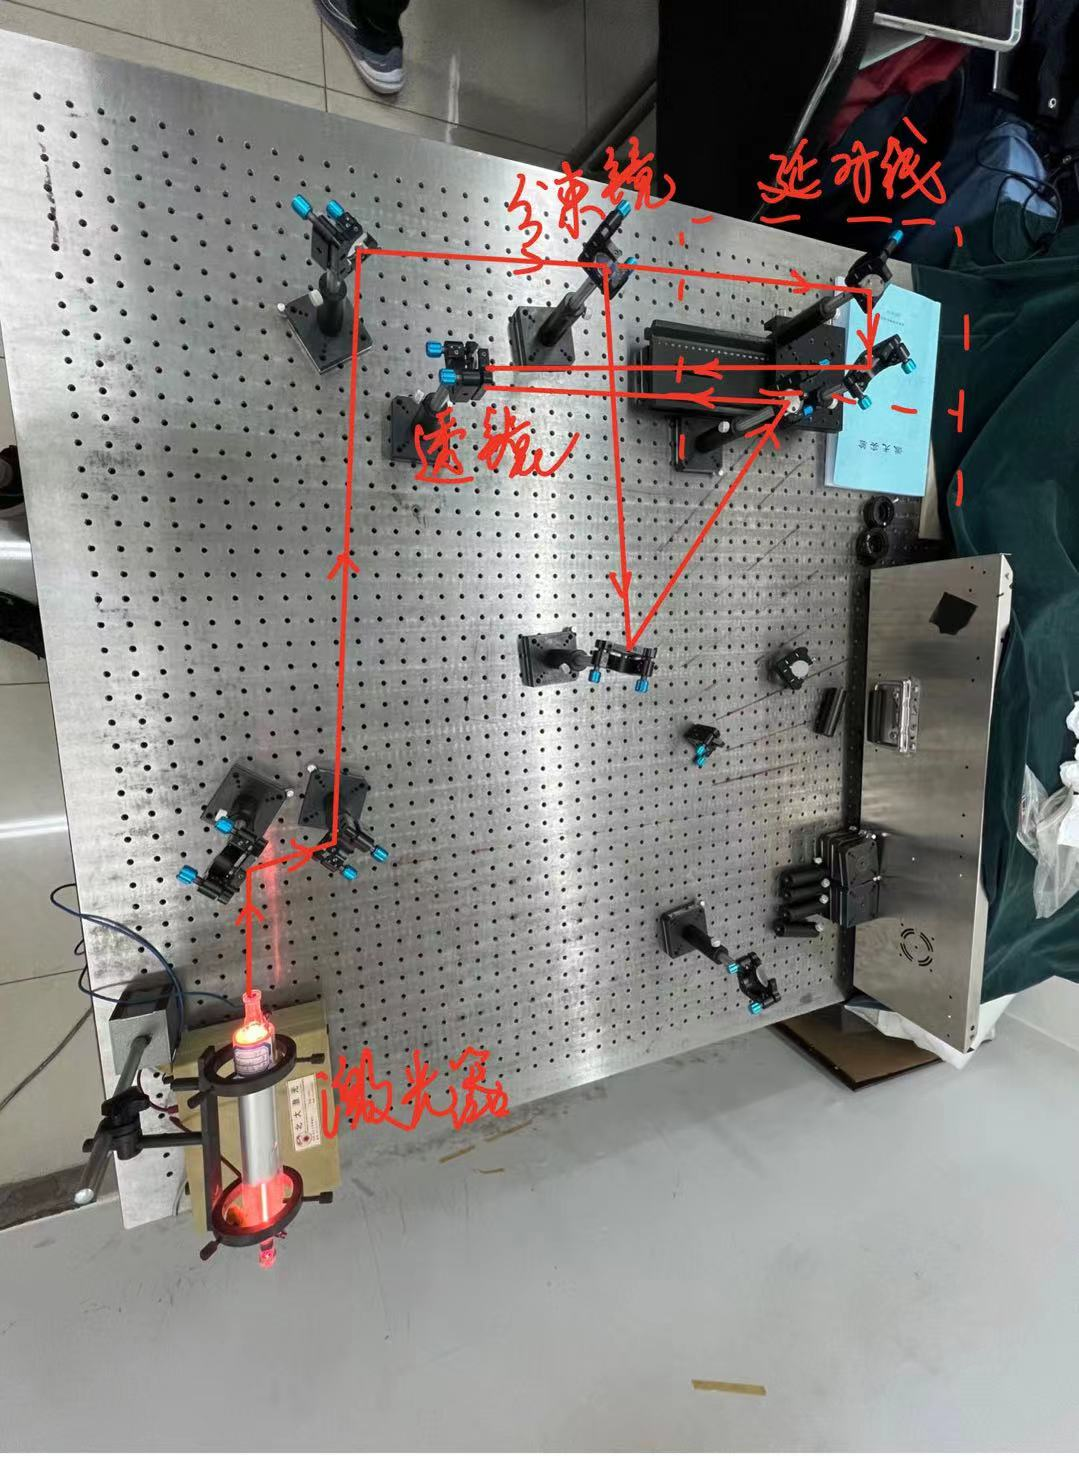
\includegraphics[width=.8\linewidth]{img/2.jpg}
	\caption[实验中搭建的非共线的泵浦探测光路. 各元件均已在图中标出,未标记的均为反射镜.
    ]{实验中搭建的非共线的泵浦探测光路. 各元件均已在图中标出,未标记的均为反射镜.
    }\vspace{1ex}
	\end{figure}
    \par 实验搭建的光路如图2所示. 下面依照光线从前往后的顺序介绍各自的功能.
    \par 激光经He-Ne激光器出射.光路中最前面的三个反射镜用于调节光线的高度, 并让其与光学平台平行; 调节平行的方法是让反射镜与小孔光阑相距较远和较近的时候光都能通过小孔, 具体来说就是, 在反射镜与光阑较远时, 调节反射镜仰角使得光通过小孔, 然后让光阑与反射镜较近,调节光阑高度让光线通过小孔, 如此反复几次便能调好; 此时小孔光阑的高度也与光线高度一致, 之后在引入新的元件的时候只需调节这个元件使得经过这个元件的光线的高度与小孔一致, 这便保证了光线与平台平行.
    \par 光线经过前三个反射镜后经过分束镜之后分成两束;选较强的一束(本实验中即为反射光)作为泵浦光, 让其经过两个反射镜后到达透镜和样品. 中间加的两个反射镜作用是增加光程, 便于延时线零点的寻找.
    \par 经过分束镜的透射光用于探测. 其经过两个反射镜组成的延时线后到达透镜和样品. 通过调节延时线上的两个反射镜便可以调节探测光的光程, 从而调节泵浦光与探测光到达样品的时间差, 从而探测超快动力学过程.
    \par 实验中延时线放的位置基本上是时间延迟的零点, 即图中位形下泵浦光和探测光到达样品的光程基本相等(差距约为cm量级). 并且此时泵浦光和探测光相交于样品面. 探测时将样品放于样品面处, 然后在后面探测光的前方放上探测器即可进行探测; 通过改变时延线即可探测动力学过程.
    \par 具体实验中需要根据所研究的动力学过程考虑调节时延线所用的方法.比如说1ns时间差对应光程差为0.3m, 调节精度在cm量级即可; 但1ps时间差对应路程差为0.3mm, 调节时便需要使用能够精细调节几十$\mu m$乃至几$\mu m$的设备. 此外, 时延线也要先预调整使得泵浦光和探测光大致光程已经相等, 这有助于精细地寻找时间零点.
\section{结论}
%	首先要给出实验结果,然后再给出由实验结果分析得到的结果和结论.此部分给出的内容要比摘要中的全面,用词要更准确.\par
本实验中实现了一种非共线泵浦-探测光路的搭建, 实现了可调节的时延线, 并估计好了样品要放置的位置, 从而为超快动力学过程的探测提供了光路, 为以后类似的实验提供了训练和思路.
\section{思考题}
1.在设计泵浦探测光路时,都需要考虑哪些重要因素,实验的难点在哪里?为什么必须找到时间重合的零点? 
\par 答:(1)设计泵浦探测光路时需要考虑实验中允许使用的空间, 对光源发出的光进行调节所需的元件, 该使用共线探测还是非共线探测, 所研究的动力学时间尺度, 调节时延线的方法, 样品中所研究现象开始出现的光强等等因素, 从而选择具有合适脉宽和重复度的脉冲激光器等等光学元件.

(2)实验中难点在于对于时间重合零点的寻找. 如果探测的是吸收谱,则改变时延线过程中吸收谱原吸收峰变弱或者出现新的吸收峰标志着时间零点的到达; 针对所要研究的效应, 会有不同的时间零点到达的判据. 

(3)因为所要研究的动力学过程开始于泵浦激光的激发. 因而研究的起点便是时间重合的零点, 因而必须找到零点.

2.请设计一个测量脉冲宽度为10fs、波长为830nm的飞秒激光的脉冲宽度的方法。
\par 答:利用自相关测量探测方法(如图所示), 通过探测两束光的二阶自相关可以分析得到脉宽的信息. 由于飞秒激光脉宽很窄, 不能使用延时线, 一种解决方法就如图所示, 由于两束光在KDP晶体内非共线, 因而空间上的分布反映了时间上的不同, 从而相当于探测了不同时间差的自相关信号, 对信号分析便可得到脉宽.
	\begin{figure}[!h]
	\centering
	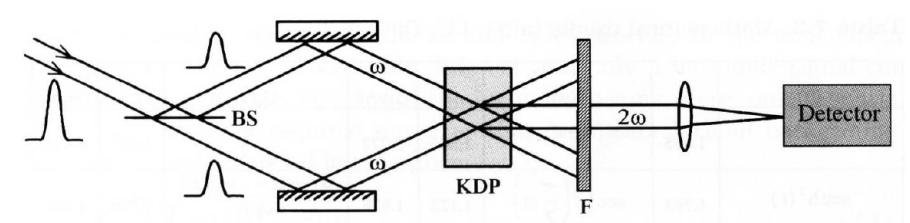
\includegraphics[width=.8\linewidth]{img/3.png}
	\caption[单脉冲非共线干涉自相关仪的原理示意图]{单脉冲非共线干涉自相关仪的原理示意图}\vspace{1ex}
	\end{figure}
\section{致谢}
%	此部分感谢同组人...和对实验和报告有帮助的人.
	感谢我的合作伙伴杨轩同学,他的工作是不可或缺的;感谢耐心的胡小永指导老师对我们的巨大帮助。
\begin{thebibliography}{99}
	\addcontentsline{toc}{section}{参考文献}
	\bibitem{ref1}北京大学物理学院光学所, 激光实验, 第二版, 北京: 北京大学物理学院, 2023.
\end{thebibliography}
\clearpage
\end{document}
